% Overleaf drop-in note: upgrades after the Tuesday meeting (Kier / Vera / Simeon).
% Paste after the ``Three-dimensional flux power'' section of part2.tex, or
% % Overleaf drop-in note: upgrades after the Tuesday meeting (Kier / Vera / Simeon).
% Paste after the ``Three-dimensional flux power'' section of part2.tex, or
% % Overleaf drop-in note: upgrades after the Tuesday meeting (Kier / Vera / Simeon).
% Paste after the ``Three-dimensional flux power'' section of part2.tex, or
% % Overleaf drop-in note: upgrades after the Tuesday meeting (Kier / Vera / Simeon).
% Paste after the ``Three-dimensional flux power'' section of part2.tex, or
% \input{update_post_meeting} from the main file. Figures live in plots/.
%
% Companion script: make_full_physics_plots.py
% Figures: 15_full_physics_p1d_p3d.pdf, 16_full_physics_param_vary.pdf

\section{Post-meeting upgrade: full physics in one realisation}
\label{sec:fullphysics}

\subsection{Motivation}

The Tuesday discussion asked for $P_{1\mathrm{D}}(k_\parallel)$ and $P_F(k,\mu)$ measured from sightlines that include the same physics: lognormal density, Jeans smoothing, thermal broadening, FGPA optical depth, and peculiar velocities.
Section~\ref{sec:box} already had Jeans, lognormal, FGPA, and linear redshift-space distortions in the cube, but thermal broadening was off, and $P_{1\mathrm{D}}$ was not taken from that same volume.
The 1D FGPA sightlines of Part~I remained in real space.

\subsection{What changed relative to Figure~\ref{fig:box}}

\begin{center}
\small
\begin{tabular}{@{}lll@{}}
\toprule
Ingredient & Figure~\ref{fig:box} (meeting) & This update \\
\midrule
Jeans $x_J$ on $P_\mathrm{CDM}$ & $100\,\mathrm{kpc}/h$ & same \\
Lognormal $\Delta$ + FGPA $\tau=A\Delta^{\beta}$ & yes & same \\
Linear peculiar velocities (CIC on $\tau$) & yes & same \\
Thermal Gaussian on $\tau$ (after the shift) & off & on ($\sigma_v=10\,\mathrm{km\,s}^{-1}$ fiducial) \\
$\langle F\rangle$ & $0.696$ & same \\
$P_F(k,\mu)$ from the cube & yes & yes \\
$P_{1\mathrm{D}}$ from the same LOS skewers & no & yes \\
Parameter variations & no & $A_s$, $n_s$, $x_J$, $\sigma_{v,\mathrm{th}}$ \\
\bottomrule
\end{tabular}
\end{center}

The processing order in the cube is now
\begin{equation}
\delta_G
\;\to\;
\Delta=\mathrm{e}^{\delta_G-\sigma_G^{2}/2}
\;\to\;
\tau_\mathrm{unit}=\Delta^{\beta}
\;\to\;
\text{CIC shift by }\psi_\parallel
\;\to\;
\text{thermal smooth along the LOS}
\;\to\;
\text{solve }A\text{ so }\langle\mathrm{e}^{-A\tau}\rangle=\langle F\rangle.
\end{equation}
The thermal width is specified in $\mathrm{km\,s}^{-1}$ and converted to comoving $\mathrm{Mpc}/h$ with $H(z)/((1+z)h)$, then to pixels with the cell size $L/N$.
At $z=3$, $\sigma_v=10\,\mathrm{km\,s}^{-1}$ corresponds to $\sigma_x\approx 0.088\,\mathrm{Mpc}/h$ ($\sim 0.3$ cells on the $40\,\mathrm{Mpc}/h$, $128^{3}$ grid).

Every transverse cell provides one line-of-sight skewer.
$P_{1\mathrm{D}}$ is the ensemble periodogram of those $N^{2}$ flux-contrast skewers; $P_F(k,\mu)$ is the same 3D contrast binned in $k$ and $\mu$.
Both therefore share one seed, one Jeans length, one thermal width, and one fitted $A$.

\subsection{Fiducial measurement}

Figure~\ref{fig:fullphysics} uses the same geometry as Figure~\ref{fig:box}: $L=40\,\mathrm{Mpc}/h$, $N=128$, $z=3$, $x_J=100\,\mathrm{kpc}/h$, $\langle F\rangle=0.696$, linear growth rate $f\approx 0.982$.
The left panel is $P_{1\mathrm{D}}(k_\parallel)$ from the box skewers, with the analytic Kaiser $P_{1\mathrm{D}}$ on the Jeans-smoothed spectrum for reference.
The middle and right panels are $P_F(k,\mu)$ for $\mu<0.25$ and $\mu>0.75$, with the Part~I Kaiser formula and the published Arinyo-i-Prats $z=3$ formula overlaid (still not refitted).

\begin{figure}[htbp]
\centering
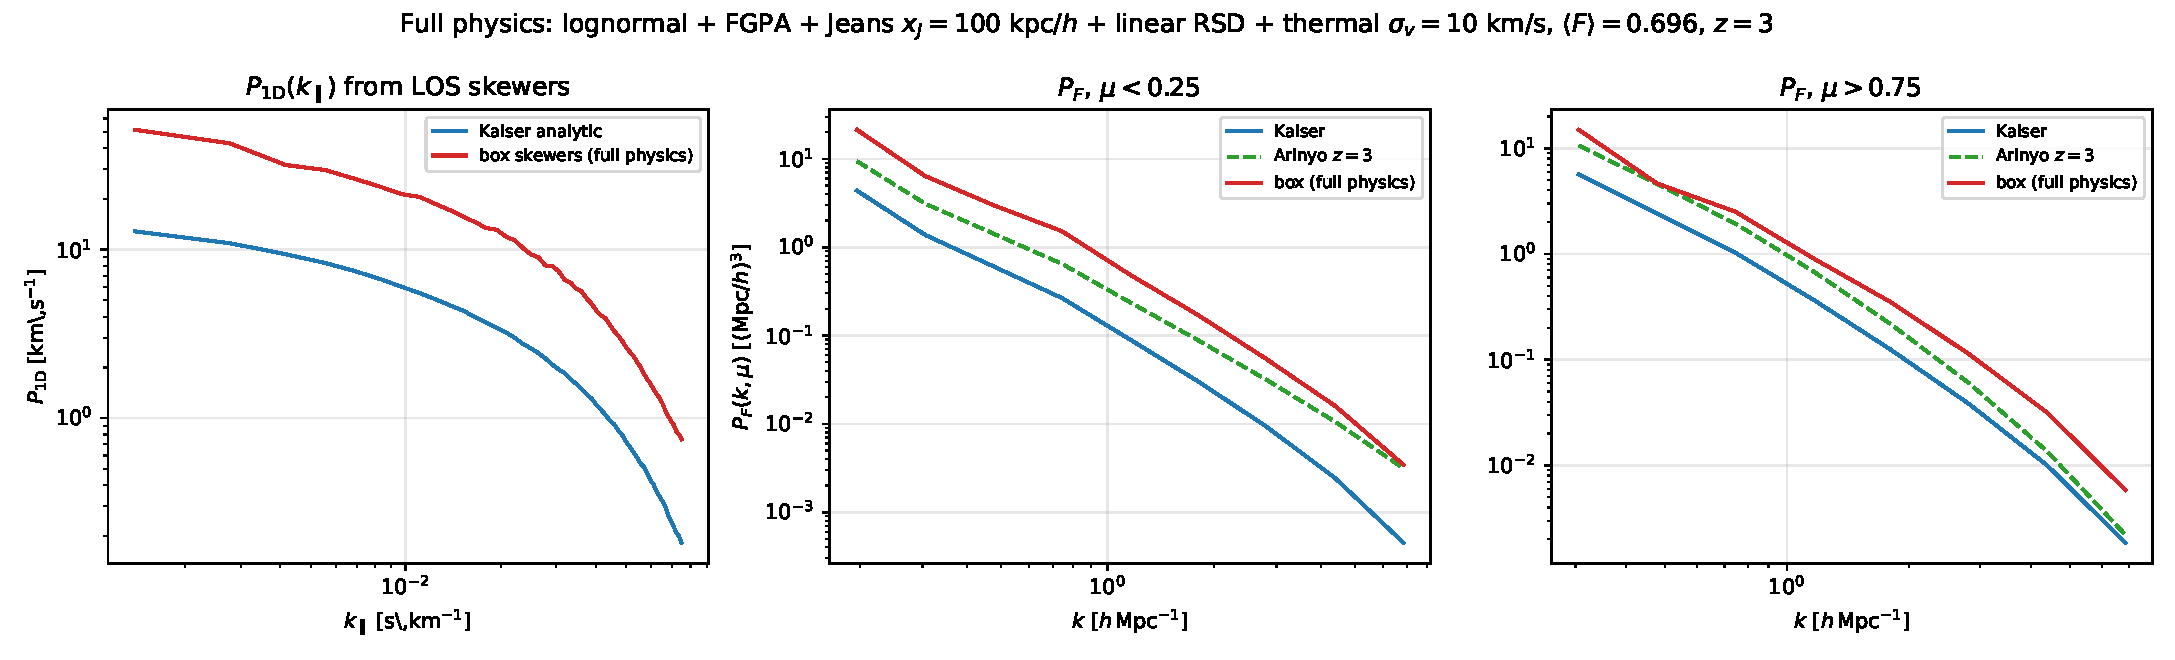
\includegraphics[width=\textwidth]{15_full_physics_p1d_p3d.pdf}
\caption{Full-physics measurement from one cube: lognormal FGPA, Jeans $x_J=100\,\mathrm{kpc}/h$, linear RSD, and thermal $\sigma_v=10\,\mathrm{km\,s}^{-1}$, at $\langle F\rangle=0.696$ and $z=3$.
Left: $P_{1\mathrm{D}}$ from all LOS skewers versus the analytic Kaiser projection.
Middle / right: $P_F(k,\mu)$ for mostly transverse and mostly parallel modes, with Kaiser and Arinyo-i-Prats overlays.}
\label{fig:fullphysics}
\end{figure}

As in Section~\ref{sec:box}, the lognormal amplitude lies above the fixed-bias Kaiser curve and above the published Arinyo formula; the slope remains closer to Arinyo than the amplitude does.
The main limits are unchanged: one small box, linear velocities only, and no refit of the Arinyo parameters.
Thermal broadening is now on, but the fiducial $10\,\mathrm{km\,s}^{-1}$ is only a fraction of a cell, so its effect is mild until $\sigma_v$ is raised (Figure~\ref{fig:paramvary}).

\subsection{Varying parameters}

Figure~\ref{fig:paramvary} repeats the full-physics cube while changing one parameter at a time, always measuring $P_{1\mathrm{D}}$ from the LOS skewers.
The four panels are $A_s$, $n_s$, the Jeans filter $\lambda_\mathrm{filter}\equiv x_J$, and the thermal width $\sigma_{v,\mathrm{th}}$.
The same random seed is kept so that changes in shape are not dominated by a new phase draw.

\begin{figure}[htbp]
\centering
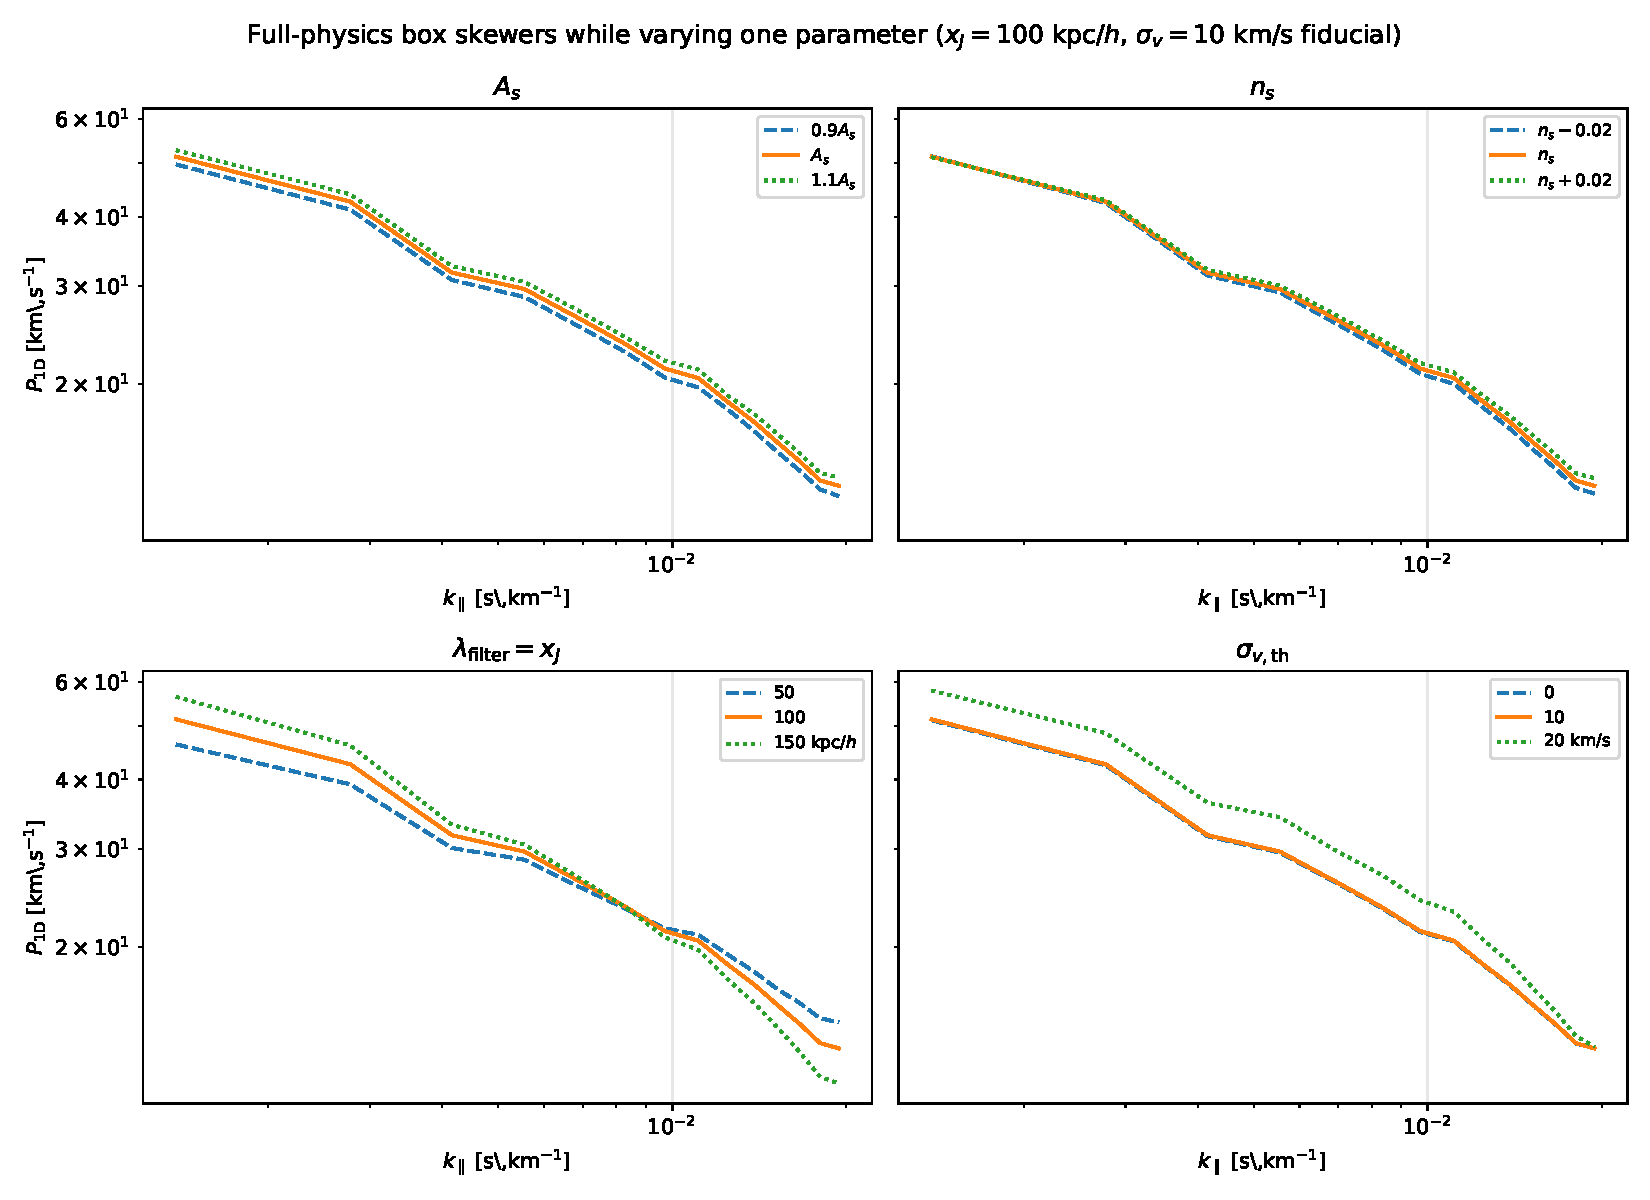
\includegraphics[width=\textwidth]{16_full_physics_param_vary.pdf}
\caption{Response of the full-physics box $P_{1\mathrm{D}}$ to one-parameter variations around the fiducial model of Figure~\ref{fig:fullphysics}.}
\label{fig:paramvary}
\end{figure}

\subsection{Code entry points}

\begin{center}
\small
\begin{tabular}{@{}p{0.42\textwidth}p{0.52\textwidth}@{}}
\toprule
Operation & Where \\
\midrule
Thermal width after RSD in the cube &
\texttt{fgpa\_flux\_box(..., thermal\_sigma\_mpch=...)} in \path{p1d/box3d.py} \\
Full-physics $P_{1\mathrm{D}}$ + $P_F(k,\mu)$ + variations &
\path{make\_full\_physics\_plots.py} \\
CLI knobs &
\texttt{--As}, \texttt{--ns}, \texttt{--lambda-filter}, \texttt{--thermal-kms}, \texttt{--mean-flux} \\
JAX twin of the pipeline (for later Fisher derivatives) &
\path{p1d\_jax/} (NumPy \path{p1d/} unchanged) \\
\bottomrule
\end{tabular}
\end{center}

Regenerate the figures with
\begin{verbatim}
python make_full_physics_plots.py
python make_full_physics_plots.py --As 2.3e-9 --ns 0.96 \
    --lambda-filter 0.1 --thermal-kms 10
\end{verbatim}
 from the main file. Figures live in plots/.
%
% Companion script: make_full_physics_plots.py
% Figures: 15_full_physics_p1d_p3d.pdf, 16_full_physics_param_vary.pdf

\section{Post-meeting upgrade: full physics in one realisation}
\label{sec:fullphysics}

\subsection{Motivation}

The Tuesday discussion asked for $P_{1\mathrm{D}}(k_\parallel)$ and $P_F(k,\mu)$ measured from sightlines that include the same physics: lognormal density, Jeans smoothing, thermal broadening, FGPA optical depth, and peculiar velocities.
Section~\ref{sec:box} already had Jeans, lognormal, FGPA, and linear redshift-space distortions in the cube, but thermal broadening was off, and $P_{1\mathrm{D}}$ was not taken from that same volume.
The 1D FGPA sightlines of Part~I remained in real space.

\subsection{What changed relative to Figure~\ref{fig:box}}

\begin{center}
\small
\begin{tabular}{@{}lll@{}}
\toprule
Ingredient & Figure~\ref{fig:box} (meeting) & This update \\
\midrule
Jeans $x_J$ on $P_\mathrm{CDM}$ & $100\,\mathrm{kpc}/h$ & same \\
Lognormal $\Delta$ + FGPA $\tau=A\Delta^{\beta}$ & yes & same \\
Linear peculiar velocities (CIC on $\tau$) & yes & same \\
Thermal Gaussian on $\tau$ (after the shift) & off & on ($\sigma_v=10\,\mathrm{km\,s}^{-1}$ fiducial) \\
$\langle F\rangle$ & $0.696$ & same \\
$P_F(k,\mu)$ from the cube & yes & yes \\
$P_{1\mathrm{D}}$ from the same LOS skewers & no & yes \\
Parameter variations & no & $A_s$, $n_s$, $x_J$, $\sigma_{v,\mathrm{th}}$ \\
\bottomrule
\end{tabular}
\end{center}

The processing order in the cube is now
\begin{equation}
\delta_G
\;\to\;
\Delta=\mathrm{e}^{\delta_G-\sigma_G^{2}/2}
\;\to\;
\tau_\mathrm{unit}=\Delta^{\beta}
\;\to\;
\text{CIC shift by }\psi_\parallel
\;\to\;
\text{thermal smooth along the LOS}
\;\to\;
\text{solve }A\text{ so }\langle\mathrm{e}^{-A\tau}\rangle=\langle F\rangle.
\end{equation}
The thermal width is specified in $\mathrm{km\,s}^{-1}$ and converted to comoving $\mathrm{Mpc}/h$ with $H(z)/((1+z)h)$, then to pixels with the cell size $L/N$.
At $z=3$, $\sigma_v=10\,\mathrm{km\,s}^{-1}$ corresponds to $\sigma_x\approx 0.088\,\mathrm{Mpc}/h$ ($\sim 0.3$ cells on the $40\,\mathrm{Mpc}/h$, $128^{3}$ grid).

Every transverse cell provides one line-of-sight skewer.
$P_{1\mathrm{D}}$ is the ensemble periodogram of those $N^{2}$ flux-contrast skewers; $P_F(k,\mu)$ is the same 3D contrast binned in $k$ and $\mu$.
Both therefore share one seed, one Jeans length, one thermal width, and one fitted $A$.

\subsection{Fiducial measurement}

Figure~\ref{fig:fullphysics} uses the same geometry as Figure~\ref{fig:box}: $L=40\,\mathrm{Mpc}/h$, $N=128$, $z=3$, $x_J=100\,\mathrm{kpc}/h$, $\langle F\rangle=0.696$, linear growth rate $f\approx 0.982$.
The left panel is $P_{1\mathrm{D}}(k_\parallel)$ from the box skewers, with the analytic Kaiser $P_{1\mathrm{D}}$ on the Jeans-smoothed spectrum for reference.
The middle and right panels are $P_F(k,\mu)$ for $\mu<0.25$ and $\mu>0.75$, with the Part~I Kaiser formula and the published Arinyo-i-Prats $z=3$ formula overlaid (still not refitted).

\begin{figure}[htbp]
\centering
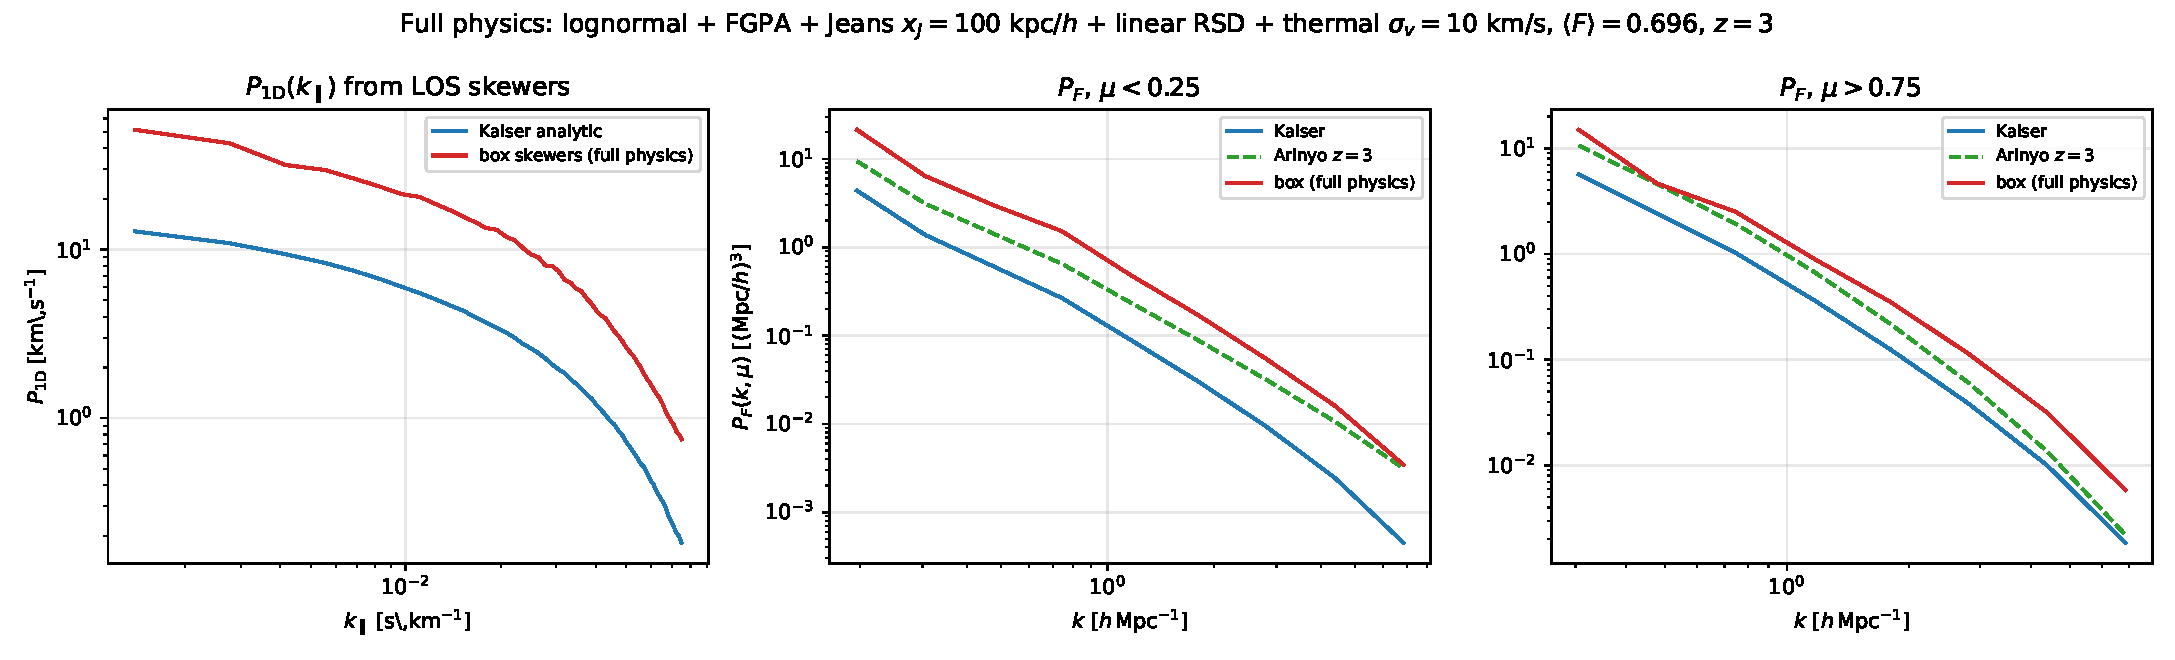
\includegraphics[width=\textwidth]{15_full_physics_p1d_p3d.pdf}
\caption{Full-physics measurement from one cube: lognormal FGPA, Jeans $x_J=100\,\mathrm{kpc}/h$, linear RSD, and thermal $\sigma_v=10\,\mathrm{km\,s}^{-1}$, at $\langle F\rangle=0.696$ and $z=3$.
Left: $P_{1\mathrm{D}}$ from all LOS skewers versus the analytic Kaiser projection.
Middle / right: $P_F(k,\mu)$ for mostly transverse and mostly parallel modes, with Kaiser and Arinyo-i-Prats overlays.}
\label{fig:fullphysics}
\end{figure}

As in Section~\ref{sec:box}, the lognormal amplitude lies above the fixed-bias Kaiser curve and above the published Arinyo formula; the slope remains closer to Arinyo than the amplitude does.
The main limits are unchanged: one small box, linear velocities only, and no refit of the Arinyo parameters.
Thermal broadening is now on, but the fiducial $10\,\mathrm{km\,s}^{-1}$ is only a fraction of a cell, so its effect is mild until $\sigma_v$ is raised (Figure~\ref{fig:paramvary}).

\subsection{Varying parameters}

Figure~\ref{fig:paramvary} repeats the full-physics cube while changing one parameter at a time, always measuring $P_{1\mathrm{D}}$ from the LOS skewers.
The four panels are $A_s$, $n_s$, the Jeans filter $\lambda_\mathrm{filter}\equiv x_J$, and the thermal width $\sigma_{v,\mathrm{th}}$.
The same random seed is kept so that changes in shape are not dominated by a new phase draw.

\begin{figure}[htbp]
\centering
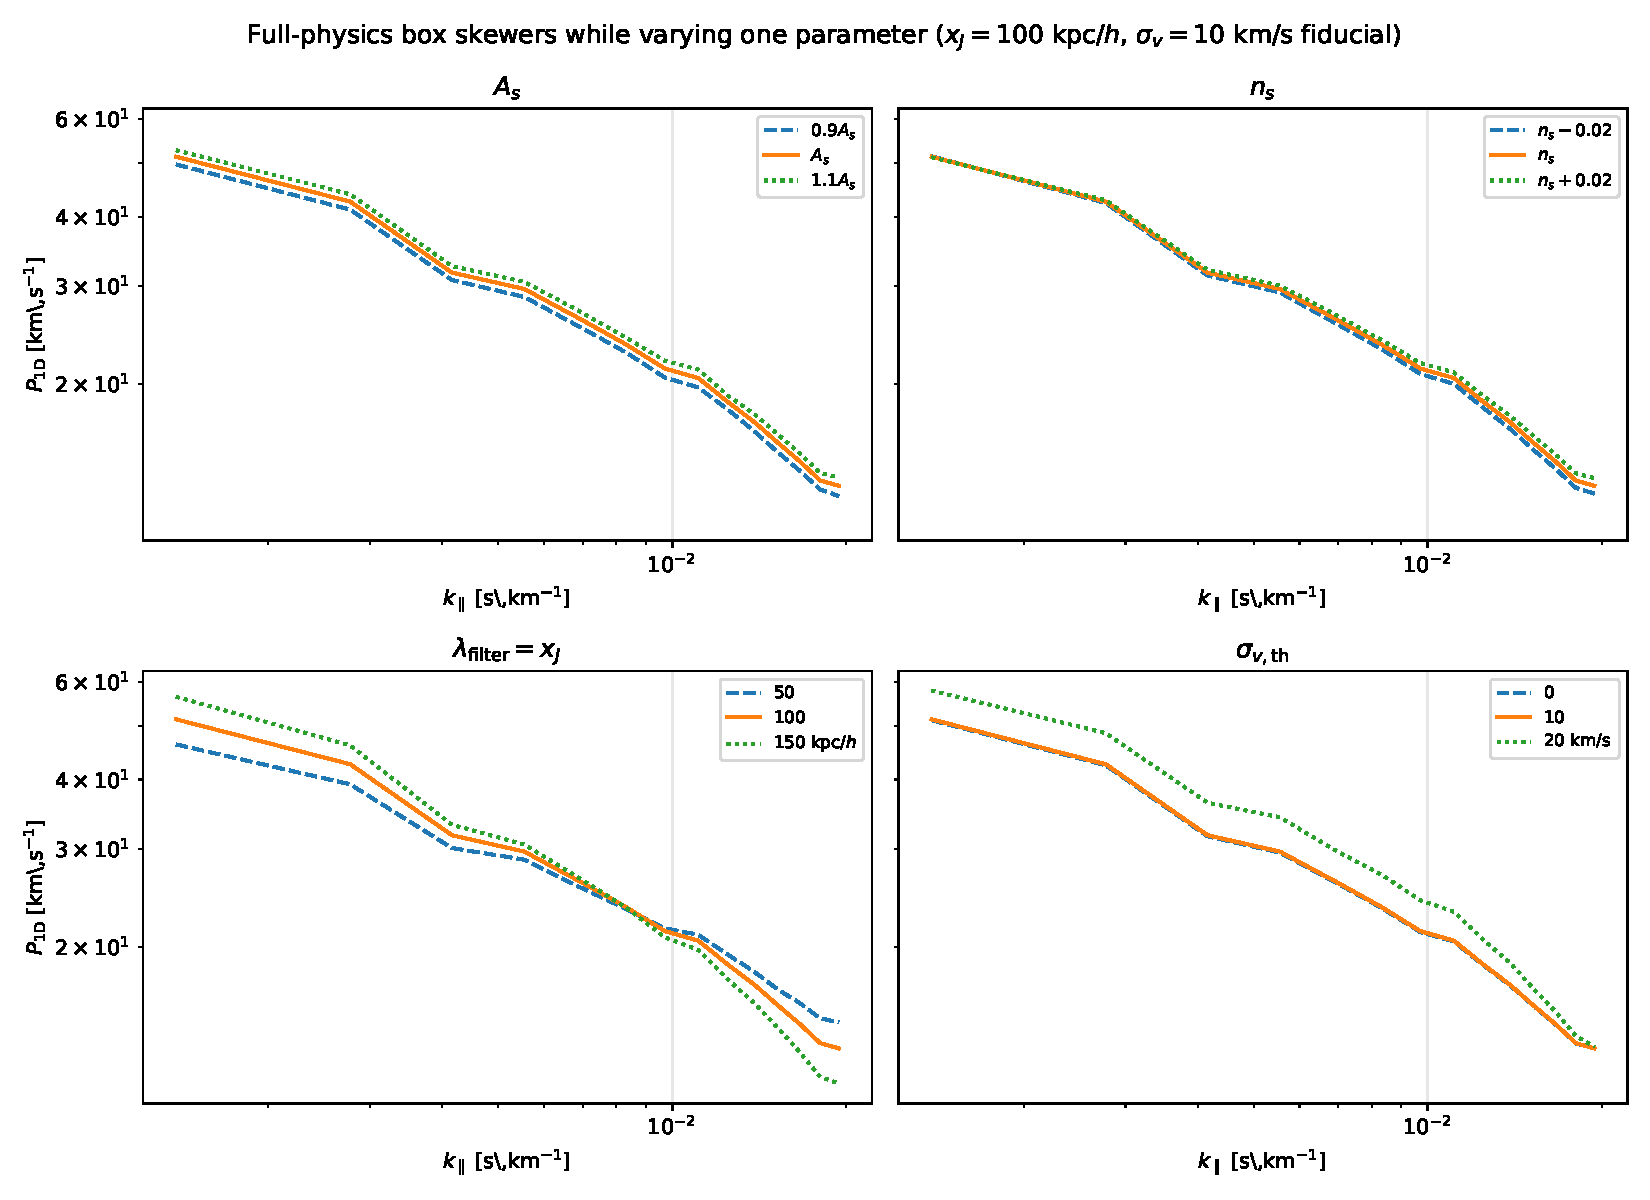
\includegraphics[width=\textwidth]{16_full_physics_param_vary.pdf}
\caption{Response of the full-physics box $P_{1\mathrm{D}}$ to one-parameter variations around the fiducial model of Figure~\ref{fig:fullphysics}.}
\label{fig:paramvary}
\end{figure}

\subsection{Code entry points}

\begin{center}
\small
\begin{tabular}{@{}p{0.42\textwidth}p{0.52\textwidth}@{}}
\toprule
Operation & Where \\
\midrule
Thermal width after RSD in the cube &
\texttt{fgpa\_flux\_box(..., thermal\_sigma\_mpch=...)} in \path{p1d/box3d.py} \\
Full-physics $P_{1\mathrm{D}}$ + $P_F(k,\mu)$ + variations &
\path{make\_full\_physics\_plots.py} \\
CLI knobs &
\texttt{--As}, \texttt{--ns}, \texttt{--lambda-filter}, \texttt{--thermal-kms}, \texttt{--mean-flux} \\
JAX twin of the pipeline (for later Fisher derivatives) &
\path{p1d\_jax/} (NumPy \path{p1d/} unchanged) \\
\bottomrule
\end{tabular}
\end{center}

Regenerate the figures with
\begin{verbatim}
python make_full_physics_plots.py
python make_full_physics_plots.py --As 2.3e-9 --ns 0.96 \
    --lambda-filter 0.1 --thermal-kms 10
\end{verbatim}
 from the main file. Figures live in plots/.
%
% Companion script: make_full_physics_plots.py
% Figures: 15_full_physics_p1d_p3d.pdf, 16_full_physics_param_vary.pdf

\section{Post-meeting upgrade: full physics in one realisation}
\label{sec:fullphysics}

\subsection{Motivation}

The Tuesday discussion asked for $P_{1\mathrm{D}}(k_\parallel)$ and $P_F(k,\mu)$ measured from sightlines that include the same physics: lognormal density, Jeans smoothing, thermal broadening, FGPA optical depth, and peculiar velocities.
Section~\ref{sec:box} already had Jeans, lognormal, FGPA, and linear redshift-space distortions in the cube, but thermal broadening was off, and $P_{1\mathrm{D}}$ was not taken from that same volume.
The 1D FGPA sightlines of Part~I remained in real space.

\subsection{What changed relative to Figure~\ref{fig:box}}

\begin{center}
\small
\begin{tabular}{@{}lll@{}}
\toprule
Ingredient & Figure~\ref{fig:box} (meeting) & This update \\
\midrule
Jeans $x_J$ on $P_\mathrm{CDM}$ & $100\,\mathrm{kpc}/h$ & same \\
Lognormal $\Delta$ + FGPA $\tau=A\Delta^{\beta}$ & yes & same \\
Linear peculiar velocities (CIC on $\tau$) & yes & same \\
Thermal Gaussian on $\tau$ (after the shift) & off & on ($\sigma_v=10\,\mathrm{km\,s}^{-1}$ fiducial) \\
$\langle F\rangle$ & $0.696$ & same \\
$P_F(k,\mu)$ from the cube & yes & yes \\
$P_{1\mathrm{D}}$ from the same LOS skewers & no & yes \\
Parameter variations & no & $A_s$, $n_s$, $x_J$, $\sigma_{v,\mathrm{th}}$ \\
\bottomrule
\end{tabular}
\end{center}

The processing order in the cube is now
\begin{equation}
\delta_G
\;\to\;
\Delta=\mathrm{e}^{\delta_G-\sigma_G^{2}/2}
\;\to\;
\tau_\mathrm{unit}=\Delta^{\beta}
\;\to\;
\text{CIC shift by }\psi_\parallel
\;\to\;
\text{thermal smooth along the LOS}
\;\to\;
\text{solve }A\text{ so }\langle\mathrm{e}^{-A\tau}\rangle=\langle F\rangle.
\end{equation}
The thermal width is specified in $\mathrm{km\,s}^{-1}$ and converted to comoving $\mathrm{Mpc}/h$ with $H(z)/((1+z)h)$, then to pixels with the cell size $L/N$.
At $z=3$, $\sigma_v=10\,\mathrm{km\,s}^{-1}$ corresponds to $\sigma_x\approx 0.088\,\mathrm{Mpc}/h$ ($\sim 0.3$ cells on the $40\,\mathrm{Mpc}/h$, $128^{3}$ grid).

Every transverse cell provides one line-of-sight skewer.
$P_{1\mathrm{D}}$ is the ensemble periodogram of those $N^{2}$ flux-contrast skewers; $P_F(k,\mu)$ is the same 3D contrast binned in $k$ and $\mu$.
Both therefore share one seed, one Jeans length, one thermal width, and one fitted $A$.

\subsection{Fiducial measurement}

Figure~\ref{fig:fullphysics} uses the same geometry as Figure~\ref{fig:box}: $L=40\,\mathrm{Mpc}/h$, $N=128$, $z=3$, $x_J=100\,\mathrm{kpc}/h$, $\langle F\rangle=0.696$, linear growth rate $f\approx 0.982$.
The left panel is $P_{1\mathrm{D}}(k_\parallel)$ from the box skewers, with the analytic Kaiser $P_{1\mathrm{D}}$ on the Jeans-smoothed spectrum for reference.
The middle and right panels are $P_F(k,\mu)$ for $\mu<0.25$ and $\mu>0.75$, with the Part~I Kaiser formula and the published Arinyo-i-Prats $z=3$ formula overlaid (still not refitted).

\begin{figure}[htbp]
\centering
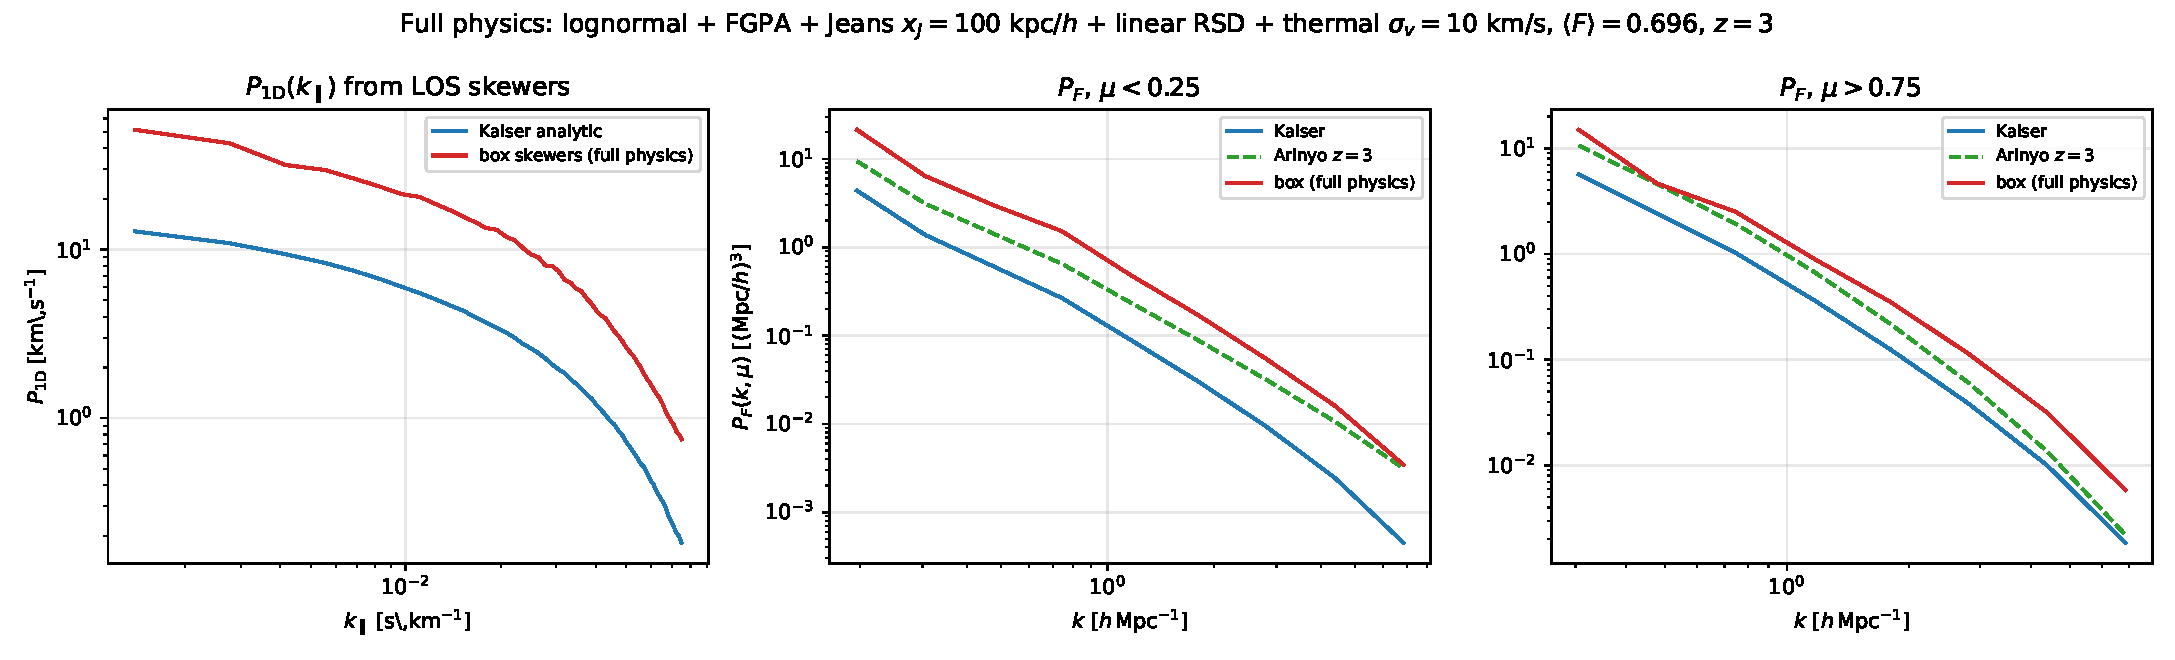
\includegraphics[width=\textwidth]{15_full_physics_p1d_p3d.pdf}
\caption{Full-physics measurement from one cube: lognormal FGPA, Jeans $x_J=100\,\mathrm{kpc}/h$, linear RSD, and thermal $\sigma_v=10\,\mathrm{km\,s}^{-1}$, at $\langle F\rangle=0.696$ and $z=3$.
Left: $P_{1\mathrm{D}}$ from all LOS skewers versus the analytic Kaiser projection.
Middle / right: $P_F(k,\mu)$ for mostly transverse and mostly parallel modes, with Kaiser and Arinyo-i-Prats overlays.}
\label{fig:fullphysics}
\end{figure}

As in Section~\ref{sec:box}, the lognormal amplitude lies above the fixed-bias Kaiser curve and above the published Arinyo formula; the slope remains closer to Arinyo than the amplitude does.
The main limits are unchanged: one small box, linear velocities only, and no refit of the Arinyo parameters.
Thermal broadening is now on, but the fiducial $10\,\mathrm{km\,s}^{-1}$ is only a fraction of a cell, so its effect is mild until $\sigma_v$ is raised (Figure~\ref{fig:paramvary}).

\subsection{Varying parameters}

Figure~\ref{fig:paramvary} repeats the full-physics cube while changing one parameter at a time, always measuring $P_{1\mathrm{D}}$ from the LOS skewers.
The four panels are $A_s$, $n_s$, the Jeans filter $\lambda_\mathrm{filter}\equiv x_J$, and the thermal width $\sigma_{v,\mathrm{th}}$.
The same random seed is kept so that changes in shape are not dominated by a new phase draw.

\begin{figure}[htbp]
\centering
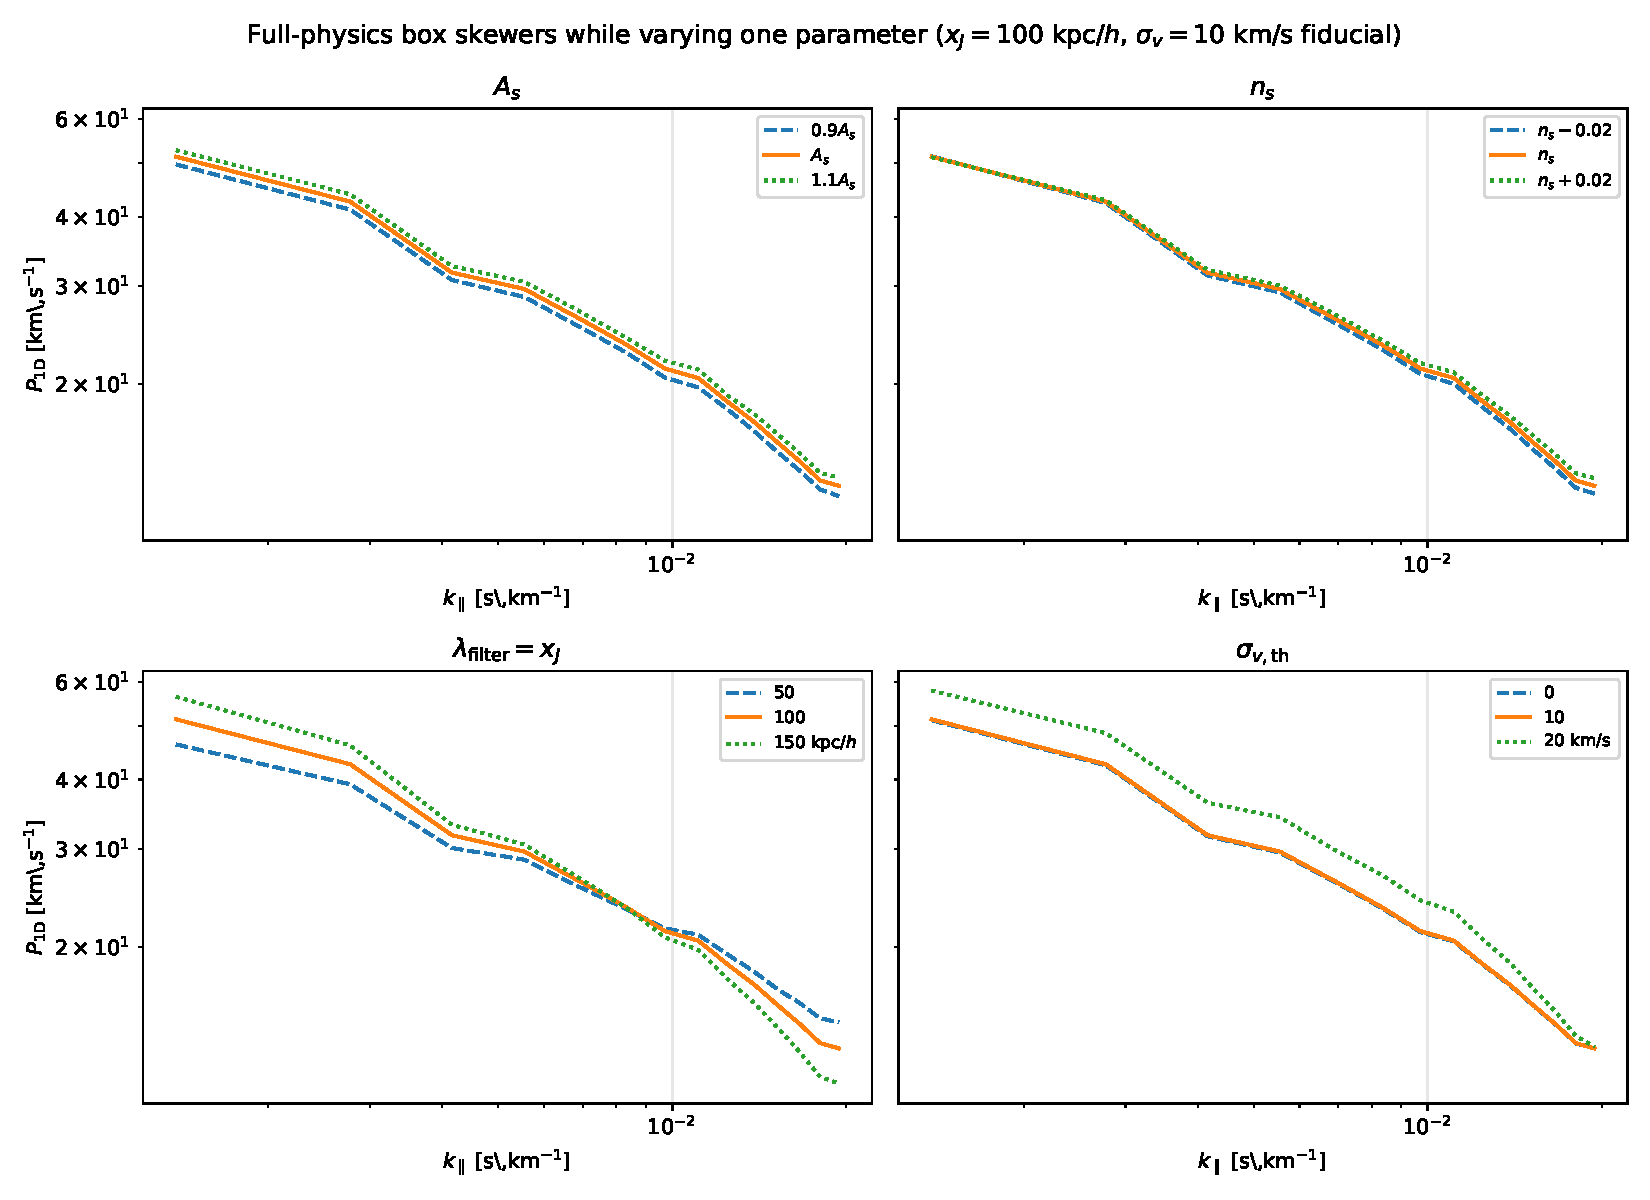
\includegraphics[width=\textwidth]{16_full_physics_param_vary.pdf}
\caption{Response of the full-physics box $P_{1\mathrm{D}}$ to one-parameter variations around the fiducial model of Figure~\ref{fig:fullphysics}.}
\label{fig:paramvary}
\end{figure}

\subsection{Code entry points}

\begin{center}
\small
\begin{tabular}{@{}p{0.42\textwidth}p{0.52\textwidth}@{}}
\toprule
Operation & Where \\
\midrule
Thermal width after RSD in the cube &
\texttt{fgpa\_flux\_box(..., thermal\_sigma\_mpch=...)} in \path{p1d/box3d.py} \\
Full-physics $P_{1\mathrm{D}}$ + $P_F(k,\mu)$ + variations &
\path{make\_full\_physics\_plots.py} \\
CLI knobs &
\texttt{--As}, \texttt{--ns}, \texttt{--lambda-filter}, \texttt{--thermal-kms}, \texttt{--mean-flux} \\
JAX twin of the pipeline (for later Fisher derivatives) &
\path{p1d\_jax/} (NumPy \path{p1d/} unchanged) \\
\bottomrule
\end{tabular}
\end{center}

Regenerate the figures with
\begin{verbatim}
python make_full_physics_plots.py
python make_full_physics_plots.py --As 2.3e-9 --ns 0.96 \
    --lambda-filter 0.1 --thermal-kms 10
\end{verbatim}
 from the main file. Figures live in plots/.
%
% Companion script: make_full_physics_plots.py
% Figures: 15_full_physics_p1d_p3d.pdf, 16_full_physics_param_vary.pdf

\section{Post-meeting upgrade: full physics in one realisation}
\label{sec:fullphysics}

\subsection{Motivation}

The Tuesday discussion asked for $P_{1\mathrm{D}}(k_\parallel)$ and $P_F(k,\mu)$ measured from sightlines that include the same physics: lognormal density, Jeans smoothing, thermal broadening, FGPA optical depth, and peculiar velocities.
Section~\ref{sec:box} already had Jeans, lognormal, FGPA, and linear redshift-space distortions in the cube, but thermal broadening was off, and $P_{1\mathrm{D}}$ was not taken from that same volume.
The 1D FGPA sightlines of Part~I remained in real space.

\subsection{What changed relative to Figure~\ref{fig:box}}

\begin{center}
\small
\begin{tabular}{@{}lll@{}}
\toprule
Ingredient & Figure~\ref{fig:box} (meeting) & This update \\
\midrule
Jeans $x_J$ on $P_\mathrm{CDM}$ & $100\,\mathrm{kpc}/h$ & same \\
Lognormal $\Delta$ + FGPA $\tau=A\Delta^{\beta}$ & yes & same \\
Linear peculiar velocities (CIC on $\tau$) & yes & same \\
Thermal Gaussian on $\tau$ (after the shift) & off & on ($\sigma_v=10\,\mathrm{km\,s}^{-1}$ fiducial) \\
$\langle F\rangle$ & $0.696$ & same \\
$P_F(k,\mu)$ from the cube & yes & yes \\
$P_{1\mathrm{D}}$ from the same LOS skewers & no & yes \\
Parameter variations & no & $A_s$, $n_s$, $x_J$, $\sigma_{v,\mathrm{th}}$ \\
\bottomrule
\end{tabular}
\end{center}

The processing order in the cube is now
\begin{equation}
\delta_G
\;\to\;
\Delta=\mathrm{e}^{\delta_G-\sigma_G^{2}/2}
\;\to\;
\tau_\mathrm{unit}=\Delta^{\beta}
\;\to\;
\text{CIC shift by }\psi_\parallel
\;\to\;
\text{thermal smooth along the LOS}
\;\to\;
\text{solve }A\text{ so }\langle\mathrm{e}^{-A\tau}\rangle=\langle F\rangle.
\end{equation}
The thermal width is specified in $\mathrm{km\,s}^{-1}$ and converted to comoving $\mathrm{Mpc}/h$ with $H(z)/((1+z)h)$, then to pixels with the cell size $L/N$.
At $z=3$, $\sigma_v=10\,\mathrm{km\,s}^{-1}$ corresponds to $\sigma_x\approx 0.088\,\mathrm{Mpc}/h$ ($\sim 0.3$ cells on the $40\,\mathrm{Mpc}/h$, $128^{3}$ grid).

Every transverse cell provides one line-of-sight skewer.
$P_{1\mathrm{D}}$ is the ensemble periodogram of those $N^{2}$ flux-contrast skewers; $P_F(k,\mu)$ is the same 3D contrast binned in $k$ and $\mu$.
Both therefore share one seed, one Jeans length, one thermal width, and one fitted $A$.

\subsection{Fiducial measurement}

Figure~\ref{fig:fullphysics} uses the same geometry as Figure~\ref{fig:box}: $L=40\,\mathrm{Mpc}/h$, $N=128$, $z=3$, $x_J=100\,\mathrm{kpc}/h$, $\langle F\rangle=0.696$, linear growth rate $f\approx 0.982$.
The left panel is $P_{1\mathrm{D}}(k_\parallel)$ from the box skewers, with the analytic Kaiser $P_{1\mathrm{D}}$ on the Jeans-smoothed spectrum for reference.
The middle and right panels are $P_F(k,\mu)$ for $\mu<0.25$ and $\mu>0.75$, with the Part~I Kaiser formula and the published Arinyo-i-Prats $z=3$ formula overlaid (still not refitted).

\begin{figure}[htbp]
\centering
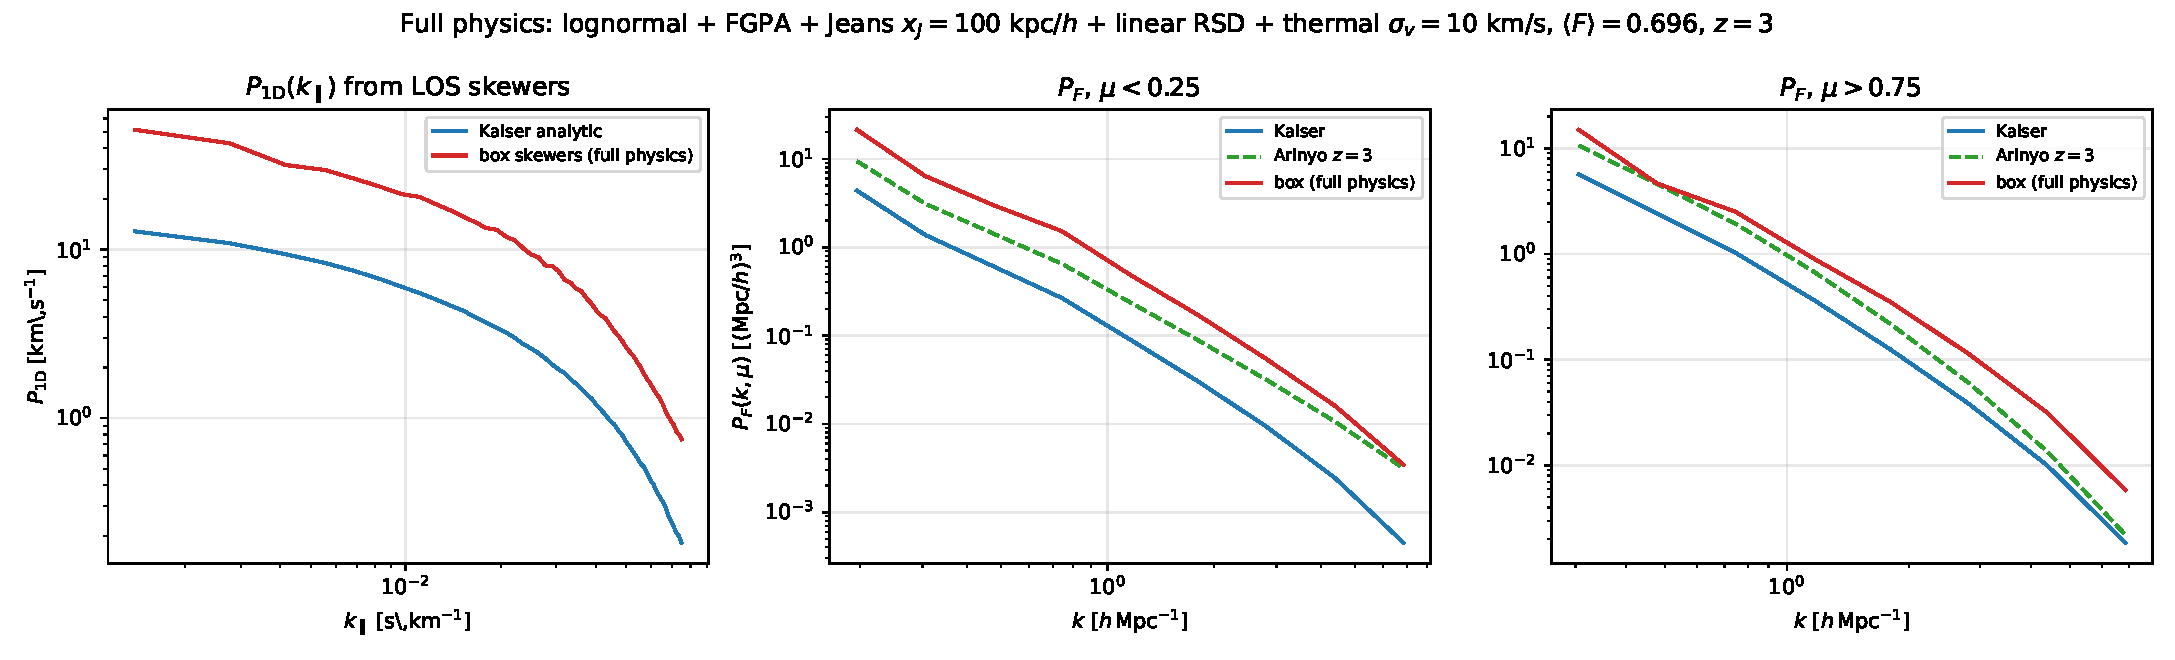
\includegraphics[width=\textwidth]{15_full_physics_p1d_p3d.pdf}
\caption{Full-physics measurement from one cube: lognormal FGPA, Jeans $x_J=100\,\mathrm{kpc}/h$, linear RSD, and thermal $\sigma_v=10\,\mathrm{km\,s}^{-1}$, at $\langle F\rangle=0.696$ and $z=3$.
Left: $P_{1\mathrm{D}}$ from all LOS skewers versus the analytic Kaiser projection.
Middle / right: $P_F(k,\mu)$ for mostly transverse and mostly parallel modes, with Kaiser and Arinyo-i-Prats overlays.}
\label{fig:fullphysics}
\end{figure}

As in Section~\ref{sec:box}, the lognormal amplitude lies above the fixed-bias Kaiser curve and above the published Arinyo formula; the slope remains closer to Arinyo than the amplitude does.
The main limits are unchanged: one small box, linear velocities only, and no refit of the Arinyo parameters.
Thermal broadening is now on, but the fiducial $10\,\mathrm{km\,s}^{-1}$ is only a fraction of a cell, so its effect is mild until $\sigma_v$ is raised (Figure~\ref{fig:paramvary}).

\subsection{Varying parameters}

Figure~\ref{fig:paramvary} repeats the full-physics cube while changing one parameter at a time, always measuring $P_{1\mathrm{D}}$ from the LOS skewers.
The four panels are $A_s$, $n_s$, the Jeans filter $\lambda_\mathrm{filter}\equiv x_J$, and the thermal width $\sigma_{v,\mathrm{th}}$.
The same random seed is kept so that changes in shape are not dominated by a new phase draw.

\begin{figure}[htbp]
\centering
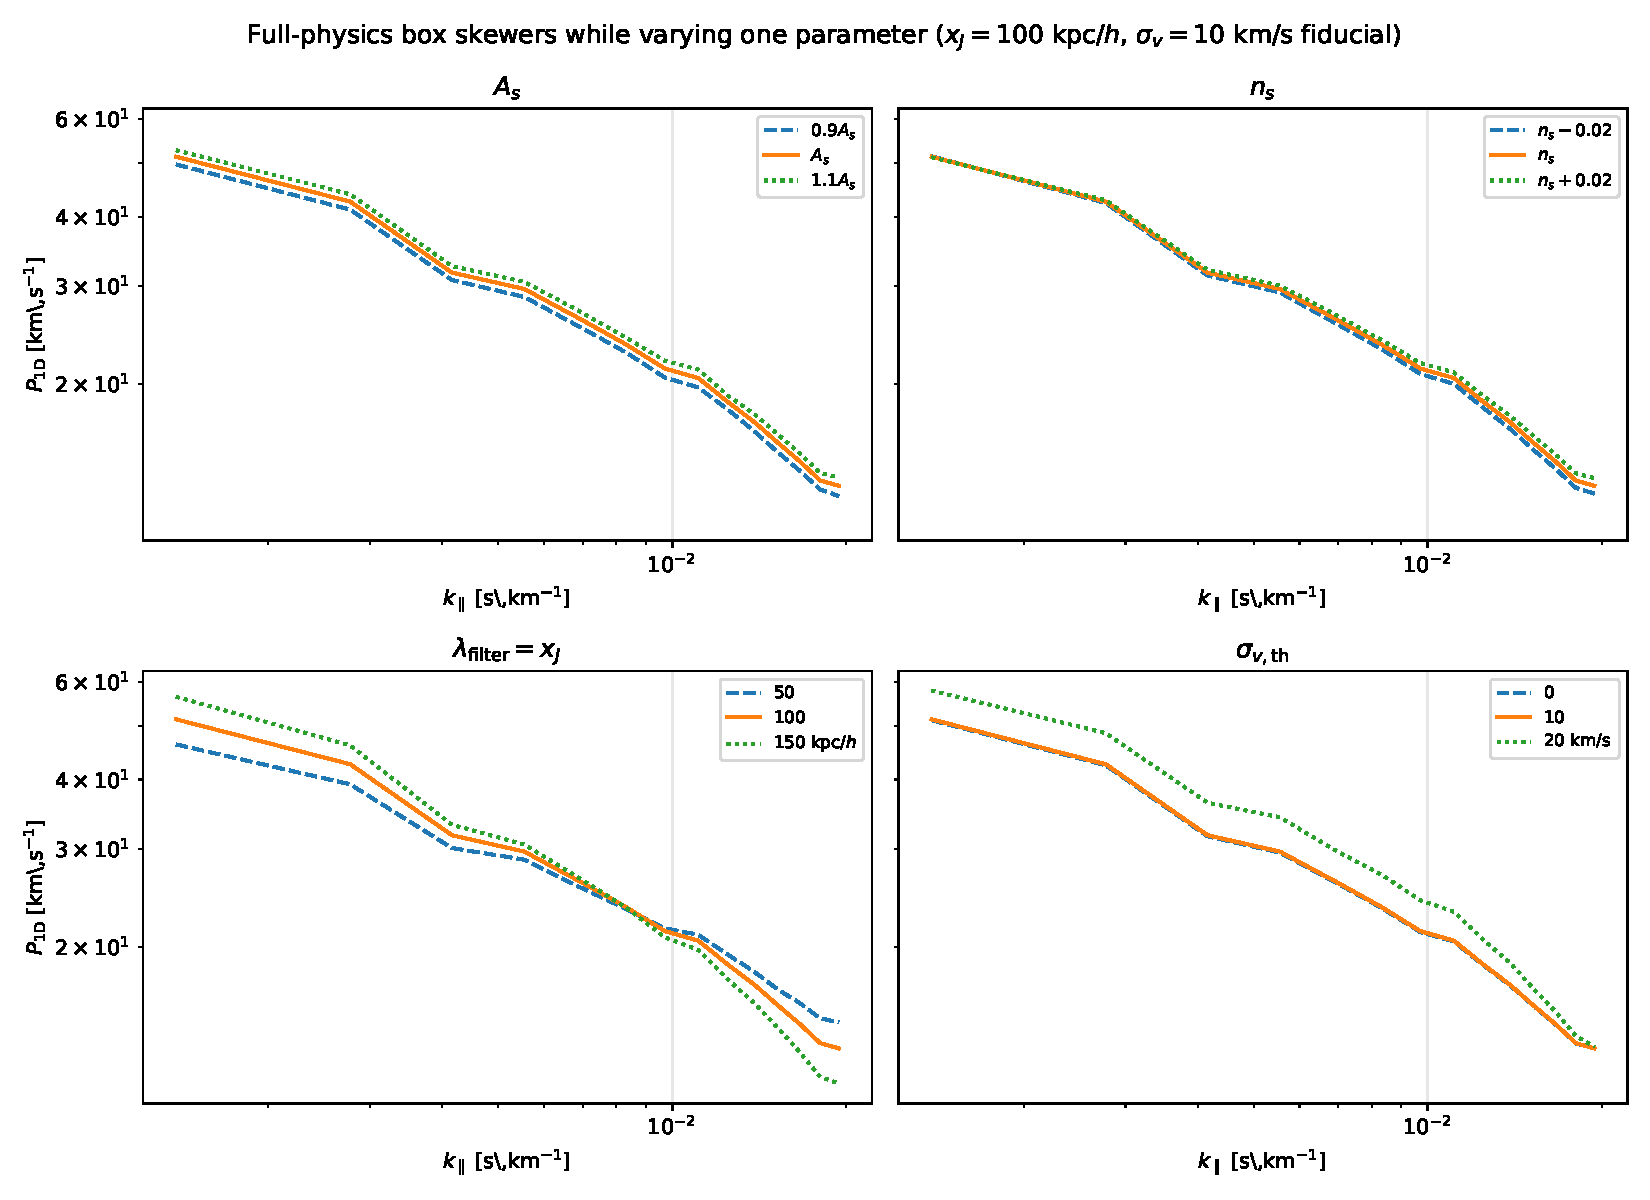
\includegraphics[width=\textwidth]{16_full_physics_param_vary.pdf}
\caption{Response of the full-physics box $P_{1\mathrm{D}}$ to one-parameter variations around the fiducial model of Figure~\ref{fig:fullphysics}.}
\label{fig:paramvary}
\end{figure}

\subsection{Code entry points}

\begin{center}
\small
\begin{tabular}{@{}p{0.42\textwidth}p{0.52\textwidth}@{}}
\toprule
Operation & Where \\
\midrule
Thermal width after RSD in the cube &
\texttt{fgpa\_flux\_box(..., thermal\_sigma\_mpch=...)} in \path{p1d/box3d.py} \\
Full-physics $P_{1\mathrm{D}}$ + $P_F(k,\mu)$ + variations &
\path{make\_full\_physics\_plots.py} \\
CLI knobs &
\texttt{--As}, \texttt{--ns}, \texttt{--lambda-filter}, \texttt{--thermal-kms}, \texttt{--mean-flux} \\
JAX twin of the pipeline (for later Fisher derivatives) &
\path{p1d\_jax/} (NumPy \path{p1d/} unchanged) \\
\bottomrule
\end{tabular}
\end{center}

Regenerate the figures with
\begin{verbatim}
python make_full_physics_plots.py
python make_full_physics_plots.py --As 2.3e-9 --ns 0.96 \
    --lambda-filter 0.1 --thermal-kms 10
\end{verbatim}
